\documentclass[14pt,letterpaper]{extarticle}
\usepackage[margin=0.6in, includehead, includefoot, headheight=18pt, headsep=0.22in, footskip=0.4in]{geometry}
\usepackage[T1]{fontenc}
\usepackage[scaled=0.95]{helvet}
\renewcommand{\familydefault}{\sfdefault}
\usepackage{tikz}
\usetikzlibrary{arrows.meta}
\usepackage{array}
\usepackage{enumitem}
\usepackage{fancyhdr}
\pagestyle{fancy}
\fancyhf{}
\fancyhead[L]{Week 9 / Bouncing paths / K--1}
\fancyfoot[L]{Bellingham Math Circle / Week 9 / F09-K-v4}
\fancyfoot[R]{\thepage}
\renewcommand{\headrulewidth}{0pt}
\renewcommand{\footrulewidth}{0pt}
\setlength{\parindent}{0pt}
\setlength{\parskip}{6pt}
\raggedright
\newcommand{\prob}[1]{\textbf{Problem #1:}}
\begin{document}
\noindent\begin{minipage}[c]{0.52\textwidth}\setlength{\parskip}{5pt}
The ball rolls on a table. It starts at the dot and rolls across the squares from corner to corner. It bounces off the walls and stops when it gets to a corner of the table. Each time it hits a wall is one bounce. Stopping at the corner is not a bounce.

Partners take turns. One puts a counter on the corner where they think the ball will stop, and the other moves a counter along the path and draws it with a crayon.
\end{minipage}\hfill
\begin{minipage}[c]{0.44\textwidth}\centering
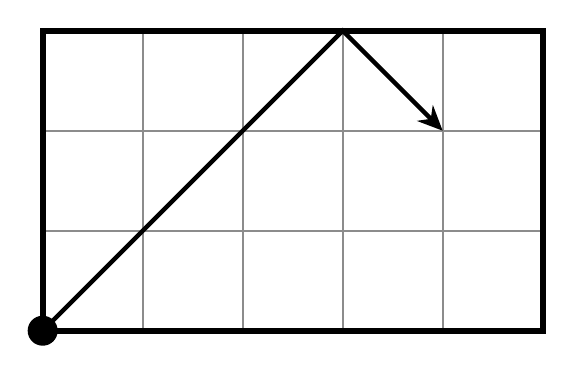
\begin{tikzpicture}[x=1in, y=1in]
\draw[black!45, line width=0.6pt] (0,0) -- (0,1.5);
\draw[black!45, line width=0.6pt] (0.5,0) -- (0.5,1.5);
\draw[black!45, line width=0.6pt] (1,0) -- (1,1.5);
\draw[black!45, line width=0.6pt] (1.5,0) -- (1.5,1.5);
\draw[black!45, line width=0.6pt] (2,0) -- (2,1.5);
\draw[black!45, line width=0.6pt] (2.5,0) -- (2.5,1.5);
\draw[black!45, line width=0.6pt] (0,0) -- (2.5,0);
\draw[black!45, line width=0.6pt] (0,0.5) -- (2.5,0.5);
\draw[black!45, line width=0.6pt] (0,1) -- (2.5,1);
\draw[black!45, line width=0.6pt] (0,1.5) -- (2.5,1.5);
\draw[line width=2.2pt] (0,0) rectangle (2.5,1.5);
\draw[line width=1.6pt, -{Stealth[length=9pt,width=8pt]}] (0,0) -- (0.5,0.5) -- (1,1) -- (1.5,1.5) -- (2,1);
\fill (0,0) circle (0.075);
\end{tikzpicture}
\end{minipage}

\vspace*{0.15in}
\prob{1} Take turns walking as the ball on the floor grid. Walk once from each dot, and draw each walk.
\begin{center}
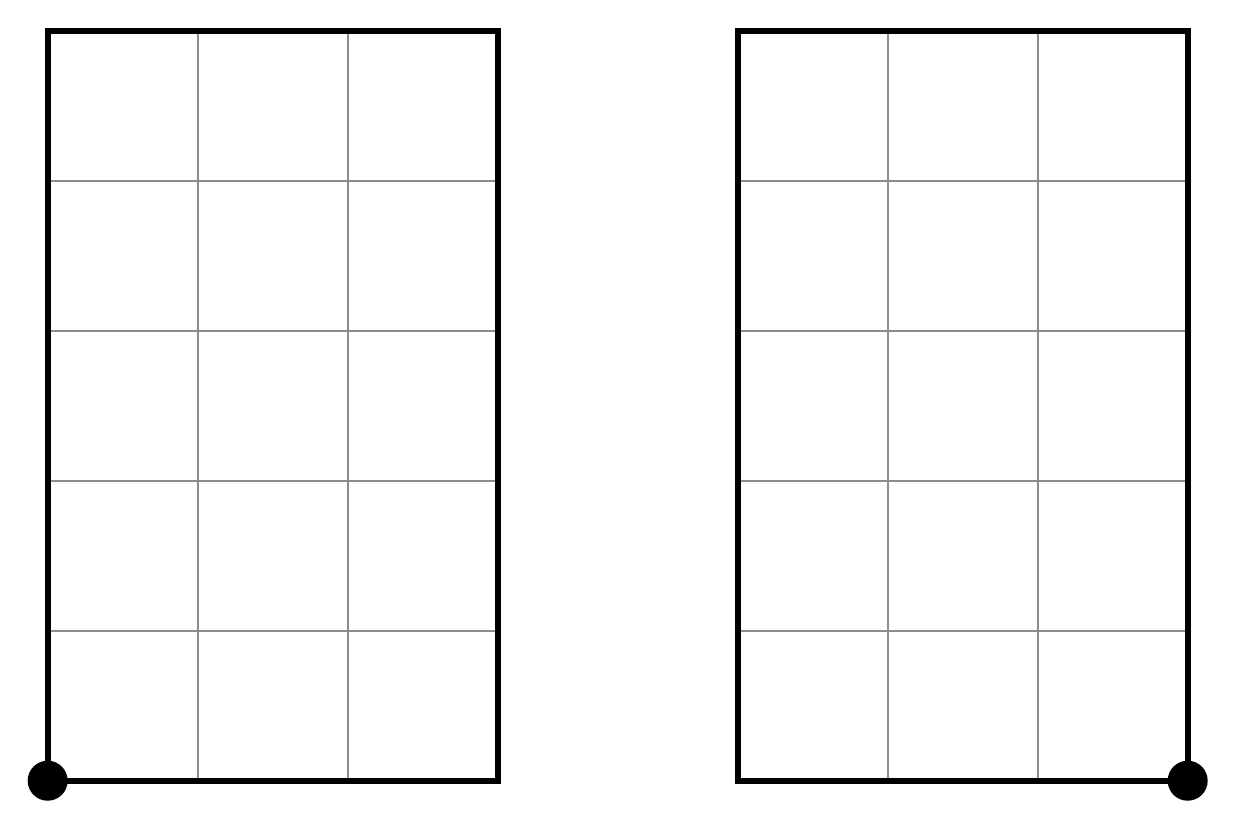
\begin{tikzpicture}[x=1in, y=1in]
\draw[black!45, line width=0.6pt] (0,0) -- (0,3.75);
\draw[black!45, line width=0.6pt] (0.75,0) -- (0.75,3.75);
\draw[black!45, line width=0.6pt] (1.5,0) -- (1.5,3.75);
\draw[black!45, line width=0.6pt] (2.25,0) -- (2.25,3.75);
\draw[black!45, line width=0.6pt] (0,0) -- (2.25,0);
\draw[black!45, line width=0.6pt] (0,0.75) -- (2.25,0.75);
\draw[black!45, line width=0.6pt] (0,1.5) -- (2.25,1.5);
\draw[black!45, line width=0.6pt] (0,2.25) -- (2.25,2.25);
\draw[black!45, line width=0.6pt] (0,3) -- (2.25,3);
\draw[black!45, line width=0.6pt] (0,3.75) -- (2.25,3.75);
\draw[line width=2.2pt] (0,0) rectangle (2.25,3.75);
\fill (0,0) circle (0.1);
\draw[black!45, line width=0.6pt] (3.45,0) -- (3.45,3.75);
\draw[black!45, line width=0.6pt] (4.2,0) -- (4.2,3.75);
\draw[black!45, line width=0.6pt] (4.95,0) -- (4.95,3.75);
\draw[black!45, line width=0.6pt] (5.7,0) -- (5.7,3.75);
\draw[black!45, line width=0.6pt] (3.45,0) -- (5.7,0);
\draw[black!45, line width=0.6pt] (3.45,0.75) -- (5.7,0.75);
\draw[black!45, line width=0.6pt] (3.45,1.5) -- (5.7,1.5);
\draw[black!45, line width=0.6pt] (3.45,2.25) -- (5.7,2.25);
\draw[black!45, line width=0.6pt] (3.45,3) -- (5.7,3);
\draw[black!45, line width=0.6pt] (3.45,3.75) -- (5.7,3.75);
\draw[line width=2.2pt] (3.45,0) rectangle (5.7,3.75);
\fill (5.7,0) circle (0.1);
\path (0,-0) rectangle (5.7,3.75);
\end{tikzpicture}
\end{center}
\newpage
\prob{2} Where does the ball stop on each table? Draw its path.
\vspace*{0.2in}
\begin{center}
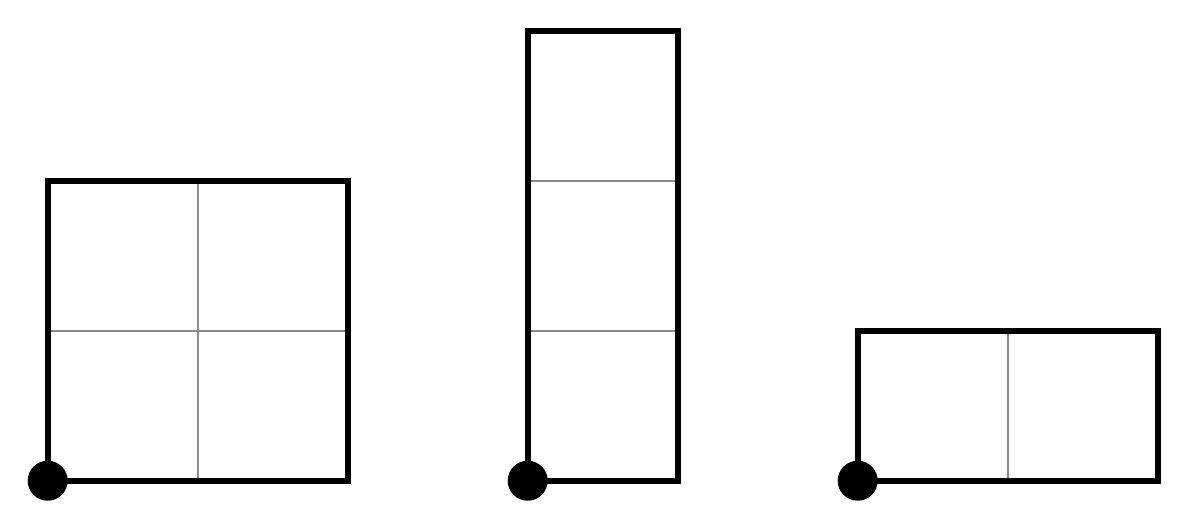
\begin{tikzpicture}[x=1in, y=1in]
\draw[black!45, line width=0.6pt] (0,0) -- (0,1.5);
\draw[black!45, line width=0.6pt] (0.75,0) -- (0.75,1.5);
\draw[black!45, line width=0.6pt] (1.5,0) -- (1.5,1.5);
\draw[black!45, line width=0.6pt] (0,0) -- (1.5,0);
\draw[black!45, line width=0.6pt] (0,0.75) -- (1.5,0.75);
\draw[black!45, line width=0.6pt] (0,1.5) -- (1.5,1.5);
\draw[line width=2.2pt] (0,0) rectangle (1.5,1.5);
\fill (0,0) circle (0.1);
\draw[black!45, line width=0.6pt] (2.4,0) -- (2.4,2.25);
\draw[black!45, line width=0.6pt] (3.15,0) -- (3.15,2.25);
\draw[black!45, line width=0.6pt] (2.4,0) -- (3.15,0);
\draw[black!45, line width=0.6pt] (2.4,0.75) -- (3.15,0.75);
\draw[black!45, line width=0.6pt] (2.4,1.5) -- (3.15,1.5);
\draw[black!45, line width=0.6pt] (2.4,2.25) -- (3.15,2.25);
\draw[line width=2.2pt] (2.4,0) rectangle (3.15,2.25);
\fill (2.4,0) circle (0.1);
\draw[black!45, line width=0.6pt] (4.05,0) -- (4.05,0.75);
\draw[black!45, line width=0.6pt] (4.8,0) -- (4.8,0.75);
\draw[black!45, line width=0.6pt] (5.55,0) -- (5.55,0.75);
\draw[black!45, line width=0.6pt] (4.05,0) -- (5.55,0);
\draw[black!45, line width=0.6pt] (4.05,0.75) -- (5.55,0.75);
\draw[line width=2.2pt] (4.05,0) rectangle (5.55,0.75);
\fill (4.05,0) circle (0.1);
\path (0,-0) rectangle (5.55,2.25);
\end{tikzpicture}
\end{center}
\vspace*{0.35in}
\begin{center}
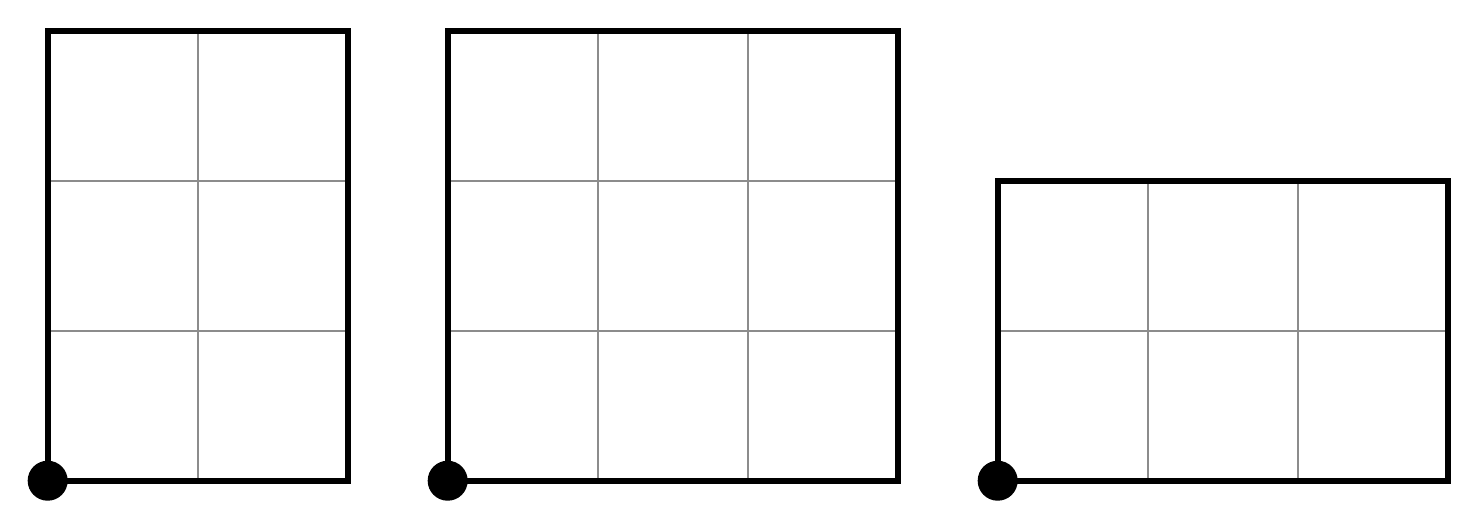
\begin{tikzpicture}[x=1in, y=1in]
\draw[black!45, line width=0.6pt] (0,0) -- (0,2.25);
\draw[black!45, line width=0.6pt] (0.75,0) -- (0.75,2.25);
\draw[black!45, line width=0.6pt] (1.5,0) -- (1.5,2.25);
\draw[black!45, line width=0.6pt] (0,0) -- (1.5,0);
\draw[black!45, line width=0.6pt] (0,0.75) -- (1.5,0.75);
\draw[black!45, line width=0.6pt] (0,1.5) -- (1.5,1.5);
\draw[black!45, line width=0.6pt] (0,2.25) -- (1.5,2.25);
\draw[line width=2.2pt] (0,0) rectangle (1.5,2.25);
\fill (0,0) circle (0.1);
\draw[black!45, line width=0.6pt] (2,0) -- (2,2.25);
\draw[black!45, line width=0.6pt] (2.75,0) -- (2.75,2.25);
\draw[black!45, line width=0.6pt] (3.5,0) -- (3.5,2.25);
\draw[black!45, line width=0.6pt] (4.25,0) -- (4.25,2.25);
\draw[black!45, line width=0.6pt] (2,0) -- (4.25,0);
\draw[black!45, line width=0.6pt] (2,0.75) -- (4.25,0.75);
\draw[black!45, line width=0.6pt] (2,1.5) -- (4.25,1.5);
\draw[black!45, line width=0.6pt] (2,2.25) -- (4.25,2.25);
\draw[line width=2.2pt] (2,0) rectangle (4.25,2.25);
\fill (2,0) circle (0.1);
\draw[black!45, line width=0.6pt] (4.75,0) -- (4.75,1.5);
\draw[black!45, line width=0.6pt] (5.5,0) -- (5.5,1.5);
\draw[black!45, line width=0.6pt] (6.25,0) -- (6.25,1.5);
\draw[black!45, line width=0.6pt] (7,0) -- (7,1.5);
\draw[black!45, line width=0.6pt] (4.75,0) -- (7,0);
\draw[black!45, line width=0.6pt] (4.75,0.75) -- (7,0.75);
\draw[black!45, line width=0.6pt] (4.75,1.5) -- (7,1.5);
\draw[line width=2.2pt] (4.75,0) rectangle (7,1.5);
\fill (4.75,0) circle (0.1);
\path (0,-0) rectangle (7,2.25);
\end{tikzpicture}
\end{center}
\newpage
\prob{3} How many times does the ball bounce on each table? Write the number in the box.
\vspace*{0.2in}
\begin{center}
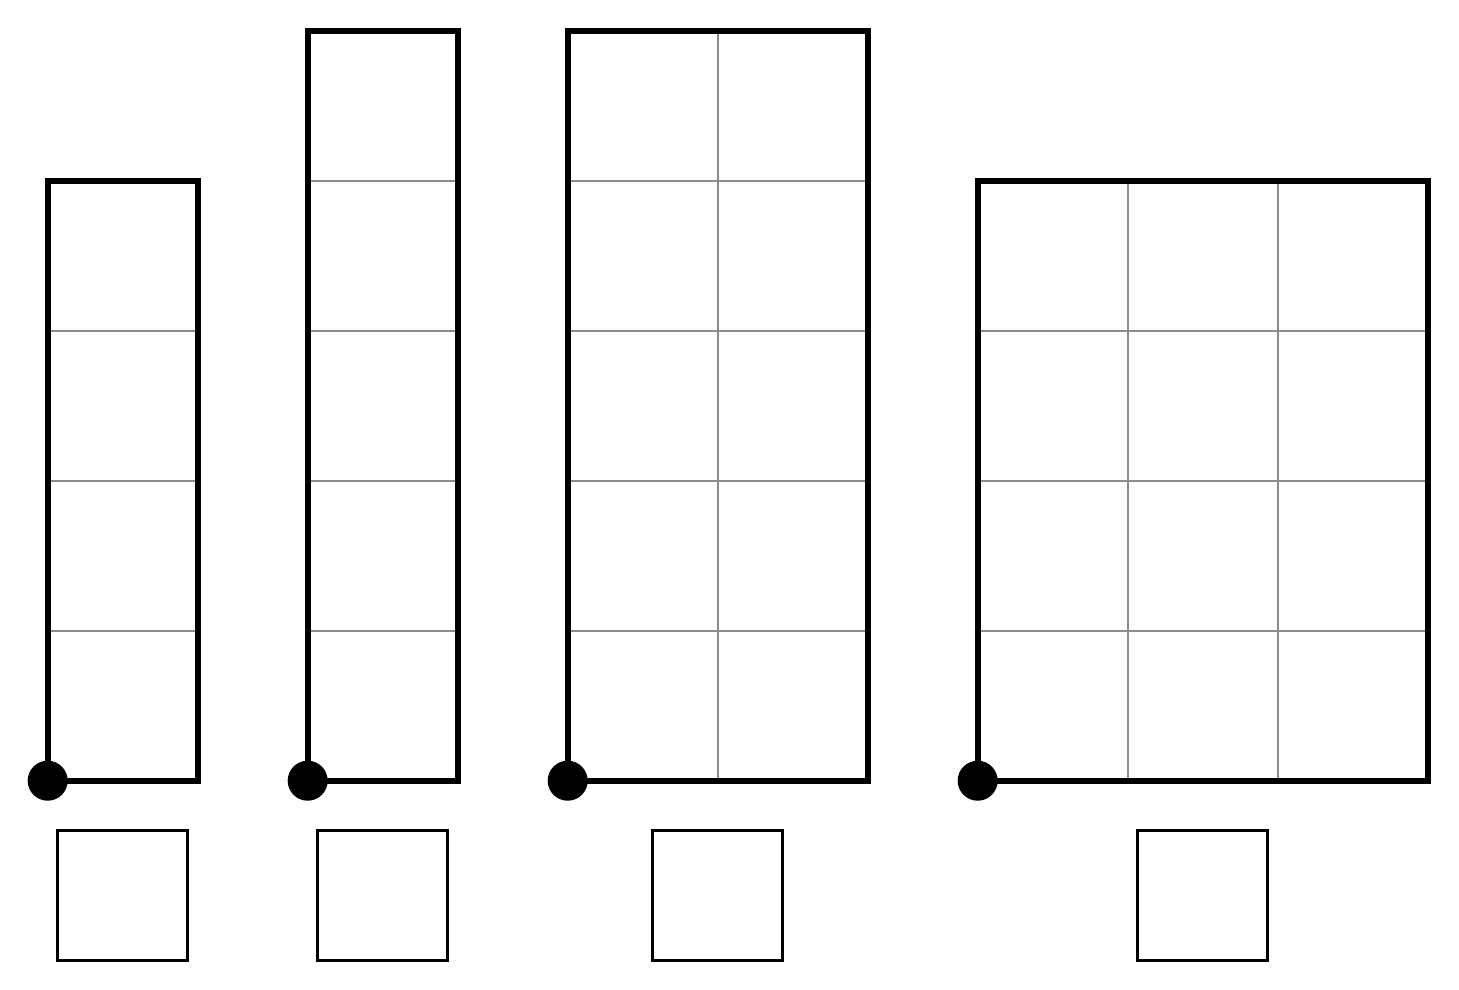
\begin{tikzpicture}[x=1in, y=1in]
\draw[black!45, line width=0.6pt] (0,0) -- (0,3);
\draw[black!45, line width=0.6pt] (0.75,0) -- (0.75,3);
\draw[black!45, line width=0.6pt] (0,0) -- (0.75,0);
\draw[black!45, line width=0.6pt] (0,0.75) -- (0.75,0.75);
\draw[black!45, line width=0.6pt] (0,1.5) -- (0.75,1.5);
\draw[black!45, line width=0.6pt] (0,2.25) -- (0.75,2.25);
\draw[black!45, line width=0.6pt] (0,3) -- (0.75,3);
\draw[line width=2.2pt] (0,0) rectangle (0.75,3);
\fill (0,0) circle (0.1);
\draw[line width=1pt] (0.05,-0.9) rectangle (0.7,-0.25);
\draw[black!45, line width=0.6pt] (1.3,0) -- (1.3,3.75);
\draw[black!45, line width=0.6pt] (2.05,0) -- (2.05,3.75);
\draw[black!45, line width=0.6pt] (1.3,0) -- (2.05,0);
\draw[black!45, line width=0.6pt] (1.3,0.75) -- (2.05,0.75);
\draw[black!45, line width=0.6pt] (1.3,1.5) -- (2.05,1.5);
\draw[black!45, line width=0.6pt] (1.3,2.25) -- (2.05,2.25);
\draw[black!45, line width=0.6pt] (1.3,3) -- (2.05,3);
\draw[black!45, line width=0.6pt] (1.3,3.75) -- (2.05,3.75);
\draw[line width=2.2pt] (1.3,0) rectangle (2.05,3.75);
\fill (1.3,0) circle (0.1);
\draw[line width=1pt] (1.35,-0.9) rectangle (2,-0.25);
\draw[black!45, line width=0.6pt] (2.6,0) -- (2.6,3.75);
\draw[black!45, line width=0.6pt] (3.35,0) -- (3.35,3.75);
\draw[black!45, line width=0.6pt] (4.1,0) -- (4.1,3.75);
\draw[black!45, line width=0.6pt] (2.6,0) -- (4.1,0);
\draw[black!45, line width=0.6pt] (2.6,0.75) -- (4.1,0.75);
\draw[black!45, line width=0.6pt] (2.6,1.5) -- (4.1,1.5);
\draw[black!45, line width=0.6pt] (2.6,2.25) -- (4.1,2.25);
\draw[black!45, line width=0.6pt] (2.6,3) -- (4.1,3);
\draw[black!45, line width=0.6pt] (2.6,3.75) -- (4.1,3.75);
\draw[line width=2.2pt] (2.6,0) rectangle (4.1,3.75);
\fill (2.6,0) circle (0.1);
\draw[line width=1pt] (3.025,-0.9) rectangle (3.675,-0.25);
\draw[black!45, line width=0.6pt] (4.65,0) -- (4.65,3);
\draw[black!45, line width=0.6pt] (5.4,0) -- (5.4,3);
\draw[black!45, line width=0.6pt] (6.15,0) -- (6.15,3);
\draw[black!45, line width=0.6pt] (6.9,0) -- (6.9,3);
\draw[black!45, line width=0.6pt] (4.65,0) -- (6.9,0);
\draw[black!45, line width=0.6pt] (4.65,0.75) -- (6.9,0.75);
\draw[black!45, line width=0.6pt] (4.65,1.5) -- (6.9,1.5);
\draw[black!45, line width=0.6pt] (4.65,2.25) -- (6.9,2.25);
\draw[black!45, line width=0.6pt] (4.65,3) -- (6.9,3);
\draw[line width=2.2pt] (4.65,0) rectangle (6.9,3);
\fill (4.65,0) circle (0.1);
\draw[line width=1pt] (5.45,-0.9) rectangle (6.1,-0.25);
\path (0,-0.9) rectangle (6.9,3.75);
\end{tikzpicture}
\end{center}
\newpage
\prob{4} Draw the path on each table. Write the number of bounces in the box.
\vspace*{0.2in}
\begin{center}
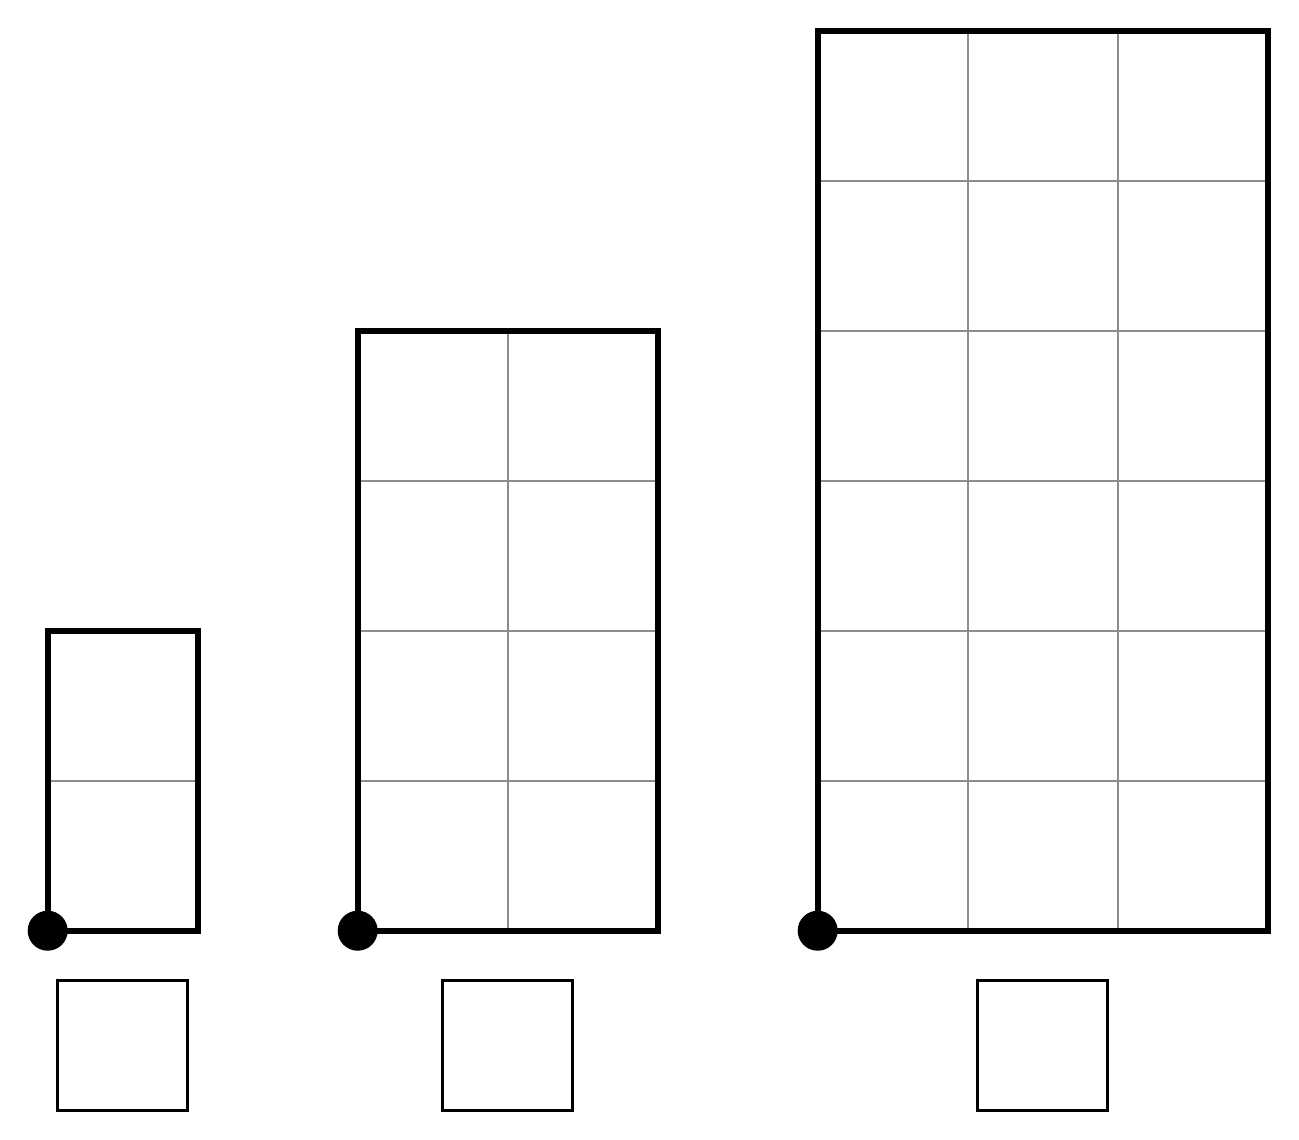
\begin{tikzpicture}[x=1in, y=1in]
\draw[black!45, line width=0.6pt] (0,0) -- (0,1.5);
\draw[black!45, line width=0.6pt] (0.75,0) -- (0.75,1.5);
\draw[black!45, line width=0.6pt] (0,0) -- (0.75,0);
\draw[black!45, line width=0.6pt] (0,0.75) -- (0.75,0.75);
\draw[black!45, line width=0.6pt] (0,1.5) -- (0.75,1.5);
\draw[line width=2.2pt] (0,0) rectangle (0.75,1.5);
\fill (0,0) circle (0.1);
\draw[line width=1pt] (0.05,-0.9) rectangle (0.7,-0.25);
\draw[black!45, line width=0.6pt] (1.55,0) -- (1.55,3);
\draw[black!45, line width=0.6pt] (2.3,0) -- (2.3,3);
\draw[black!45, line width=0.6pt] (3.05,0) -- (3.05,3);
\draw[black!45, line width=0.6pt] (1.55,0) -- (3.05,0);
\draw[black!45, line width=0.6pt] (1.55,0.75) -- (3.05,0.75);
\draw[black!45, line width=0.6pt] (1.55,1.5) -- (3.05,1.5);
\draw[black!45, line width=0.6pt] (1.55,2.25) -- (3.05,2.25);
\draw[black!45, line width=0.6pt] (1.55,3) -- (3.05,3);
\draw[line width=2.2pt] (1.55,0) rectangle (3.05,3);
\fill (1.55,0) circle (0.1);
\draw[line width=1pt] (1.975,-0.9) rectangle (2.625,-0.25);
\draw[black!45, line width=0.6pt] (3.85,0) -- (3.85,4.5);
\draw[black!45, line width=0.6pt] (4.6,0) -- (4.6,4.5);
\draw[black!45, line width=0.6pt] (5.35,0) -- (5.35,4.5);
\draw[black!45, line width=0.6pt] (6.1,0) -- (6.1,4.5);
\draw[black!45, line width=0.6pt] (3.85,0) -- (6.1,0);
\draw[black!45, line width=0.6pt] (3.85,0.75) -- (6.1,0.75);
\draw[black!45, line width=0.6pt] (3.85,1.5) -- (6.1,1.5);
\draw[black!45, line width=0.6pt] (3.85,2.25) -- (6.1,2.25);
\draw[black!45, line width=0.6pt] (3.85,3) -- (6.1,3);
\draw[black!45, line width=0.6pt] (3.85,3.75) -- (6.1,3.75);
\draw[black!45, line width=0.6pt] (3.85,4.5) -- (6.1,4.5);
\draw[line width=2.2pt] (3.85,0) rectangle (6.1,4.5);
\fill (3.85,0) circle (0.1);
\draw[line width=1pt] (4.65,-0.9) rectangle (5.3,-0.25);
\path (0,-0.9) rectangle (6.1,4.5);
\end{tikzpicture}
\end{center}
\newpage
\vspace*{0.3in}
\begin{center}
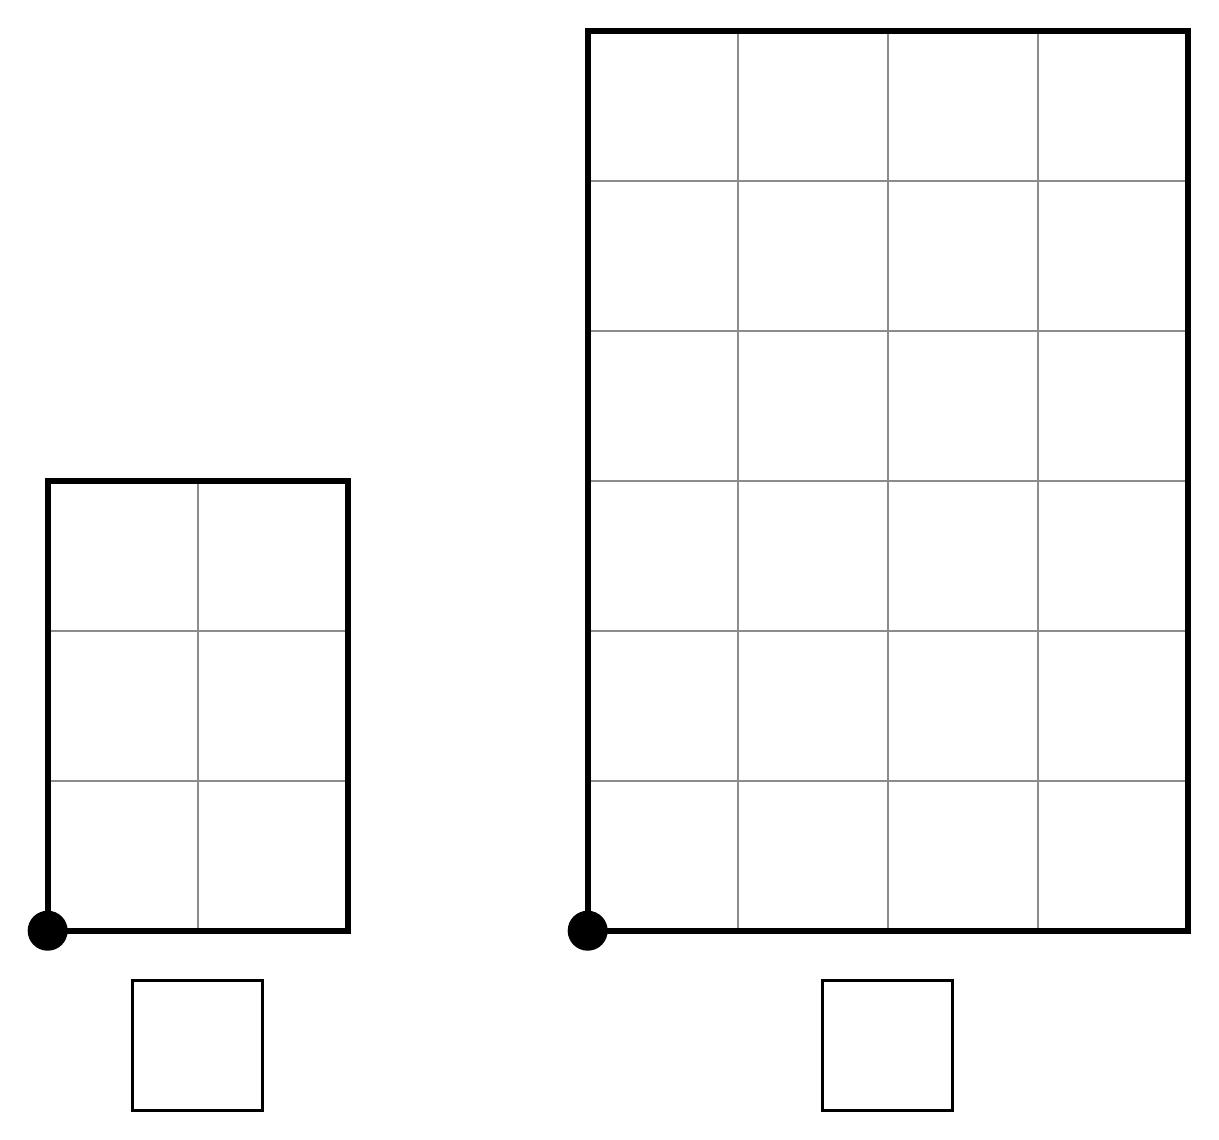
\begin{tikzpicture}[x=1in, y=1in]
\draw[black!45, line width=0.6pt] (0,0) -- (0,2.25);
\draw[black!45, line width=0.6pt] (0.75,0) -- (0.75,2.25);
\draw[black!45, line width=0.6pt] (1.5,0) -- (1.5,2.25);
\draw[black!45, line width=0.6pt] (0,0) -- (1.5,0);
\draw[black!45, line width=0.6pt] (0,0.75) -- (1.5,0.75);
\draw[black!45, line width=0.6pt] (0,1.5) -- (1.5,1.5);
\draw[black!45, line width=0.6pt] (0,2.25) -- (1.5,2.25);
\draw[line width=2.2pt] (0,0) rectangle (1.5,2.25);
\fill (0,0) circle (0.1);
\draw[line width=1pt] (0.425,-0.9) rectangle (1.075,-0.25);
\draw[black!45, line width=0.6pt] (2.7,0) -- (2.7,4.5);
\draw[black!45, line width=0.6pt] (3.45,0) -- (3.45,4.5);
\draw[black!45, line width=0.6pt] (4.2,0) -- (4.2,4.5);
\draw[black!45, line width=0.6pt] (4.95,0) -- (4.95,4.5);
\draw[black!45, line width=0.6pt] (5.7,0) -- (5.7,4.5);
\draw[black!45, line width=0.6pt] (2.7,0) -- (5.7,0);
\draw[black!45, line width=0.6pt] (2.7,0.75) -- (5.7,0.75);
\draw[black!45, line width=0.6pt] (2.7,1.5) -- (5.7,1.5);
\draw[black!45, line width=0.6pt] (2.7,2.25) -- (5.7,2.25);
\draw[black!45, line width=0.6pt] (2.7,3) -- (5.7,3);
\draw[black!45, line width=0.6pt] (2.7,3.75) -- (5.7,3.75);
\draw[black!45, line width=0.6pt] (2.7,4.5) -- (5.7,4.5);
\draw[line width=2.2pt] (2.7,0) rectangle (5.7,4.5);
\fill (2.7,0) circle (0.1);
\draw[line width=1pt] (3.875,-0.9) rectangle (4.525,-0.25);
\path (0,-0.9) rectangle (5.7,4.5);
\end{tikzpicture}
\end{center}
\newpage
\prob{5} For each little picture, draw a table starting at the dot so that the ball stops at the corner with the circle.
\begin{center}
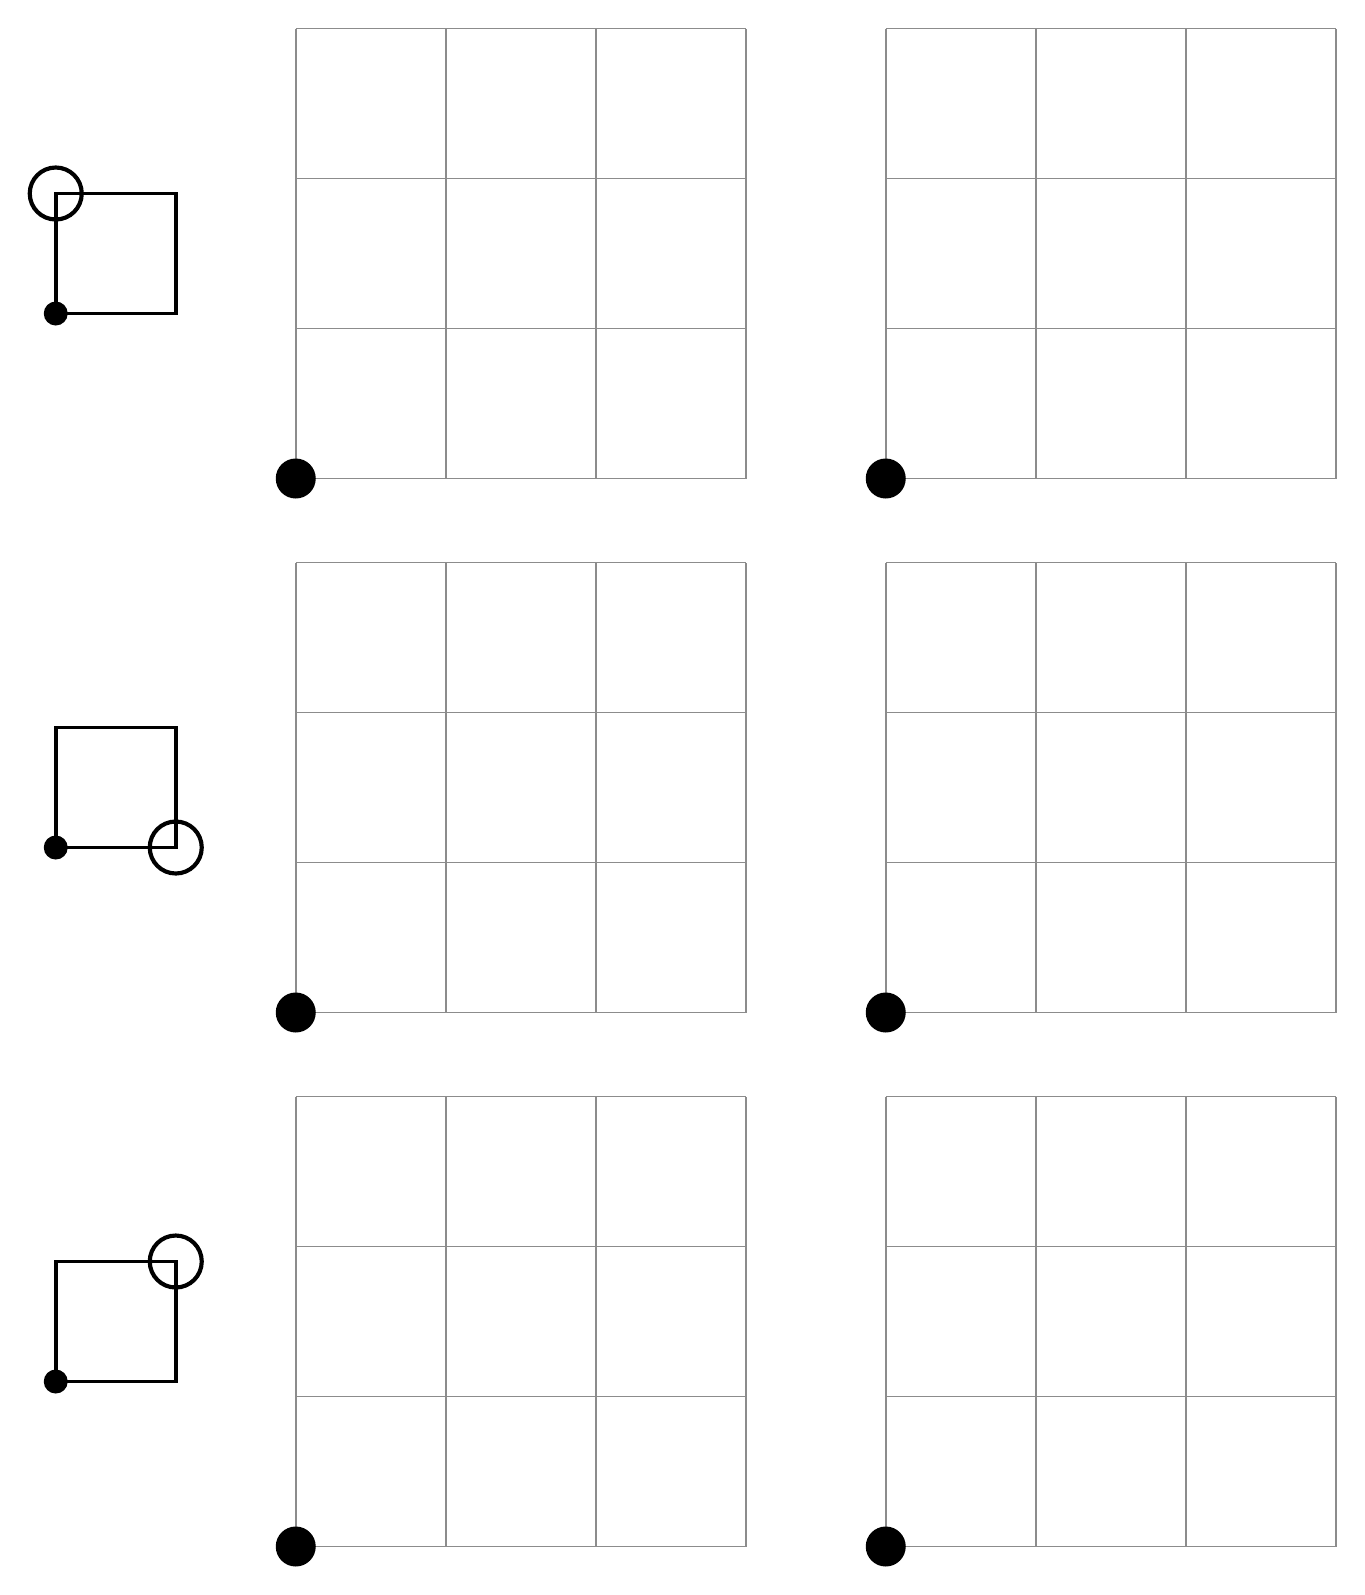
\begin{tikzpicture}[x=1in, y=1in]
\draw[line width=1.4pt] (0,-1.425) rectangle (0.6,-0.825);
\fill (0,-1.425) circle (0.06);
\draw[line width=1.5pt] (0,-0.825) circle (0.13);
\draw[black!45, line width=0.6pt] (1.2,-2.25) -- (1.2,0);
\draw[black!45, line width=0.6pt] (1.95,-2.25) -- (1.95,0);
\draw[black!45, line width=0.6pt] (2.7,-2.25) -- (2.7,0);
\draw[black!45, line width=0.6pt] (3.45,-2.25) -- (3.45,0);
\draw[black!45, line width=0.6pt] (1.2,-2.25) -- (3.45,-2.25);
\draw[black!45, line width=0.6pt] (1.2,-1.5) -- (3.45,-1.5);
\draw[black!45, line width=0.6pt] (1.2,-0.75) -- (3.45,-0.75);
\draw[black!45, line width=0.6pt] (1.2,0) -- (3.45,0);
\fill (1.2,-2.25) circle (0.1);
\draw[black!45, line width=0.6pt] (4.15,-2.25) -- (4.15,0);
\draw[black!45, line width=0.6pt] (4.9,-2.25) -- (4.9,0);
\draw[black!45, line width=0.6pt] (5.65,-2.25) -- (5.65,0);
\draw[black!45, line width=0.6pt] (6.4,-2.25) -- (6.4,0);
\draw[black!45, line width=0.6pt] (4.15,-2.25) -- (6.4,-2.25);
\draw[black!45, line width=0.6pt] (4.15,-1.5) -- (6.4,-1.5);
\draw[black!45, line width=0.6pt] (4.15,-0.75) -- (6.4,-0.75);
\draw[black!45, line width=0.6pt] (4.15,0) -- (6.4,0);
\fill (4.15,-2.25) circle (0.1);
\draw[line width=1.4pt] (0,-4.095) rectangle (0.6,-3.495);
\fill (0,-4.095) circle (0.06);
\draw[line width=1.5pt] (0.6,-4.095) circle (0.13);
\draw[black!45, line width=0.6pt] (1.2,-4.92) -- (1.2,-2.67);
\draw[black!45, line width=0.6pt] (1.95,-4.92) -- (1.95,-2.67);
\draw[black!45, line width=0.6pt] (2.7,-4.92) -- (2.7,-2.67);
\draw[black!45, line width=0.6pt] (3.45,-4.92) -- (3.45,-2.67);
\draw[black!45, line width=0.6pt] (1.2,-4.92) -- (3.45,-4.92);
\draw[black!45, line width=0.6pt] (1.2,-4.17) -- (3.45,-4.17);
\draw[black!45, line width=0.6pt] (1.2,-3.42) -- (3.45,-3.42);
\draw[black!45, line width=0.6pt] (1.2,-2.67) -- (3.45,-2.67);
\fill (1.2,-4.92) circle (0.1);
\draw[black!45, line width=0.6pt] (4.15,-4.92) -- (4.15,-2.67);
\draw[black!45, line width=0.6pt] (4.9,-4.92) -- (4.9,-2.67);
\draw[black!45, line width=0.6pt] (5.65,-4.92) -- (5.65,-2.67);
\draw[black!45, line width=0.6pt] (6.4,-4.92) -- (6.4,-2.67);
\draw[black!45, line width=0.6pt] (4.15,-4.92) -- (6.4,-4.92);
\draw[black!45, line width=0.6pt] (4.15,-4.17) -- (6.4,-4.17);
\draw[black!45, line width=0.6pt] (4.15,-3.42) -- (6.4,-3.42);
\draw[black!45, line width=0.6pt] (4.15,-2.67) -- (6.4,-2.67);
\fill (4.15,-4.92) circle (0.1);
\draw[line width=1.4pt] (0,-6.765) rectangle (0.6,-6.165);
\fill (0,-6.765) circle (0.06);
\draw[line width=1.5pt] (0.6,-6.165) circle (0.13);
\draw[black!45, line width=0.6pt] (1.2,-7.59) -- (1.2,-5.34);
\draw[black!45, line width=0.6pt] (1.95,-7.59) -- (1.95,-5.34);
\draw[black!45, line width=0.6pt] (2.7,-7.59) -- (2.7,-5.34);
\draw[black!45, line width=0.6pt] (3.45,-7.59) -- (3.45,-5.34);
\draw[black!45, line width=0.6pt] (1.2,-7.59) -- (3.45,-7.59);
\draw[black!45, line width=0.6pt] (1.2,-6.84) -- (3.45,-6.84);
\draw[black!45, line width=0.6pt] (1.2,-6.09) -- (3.45,-6.09);
\draw[black!45, line width=0.6pt] (1.2,-5.34) -- (3.45,-5.34);
\fill (1.2,-7.59) circle (0.1);
\draw[black!45, line width=0.6pt] (4.15,-7.59) -- (4.15,-5.34);
\draw[black!45, line width=0.6pt] (4.9,-7.59) -- (4.9,-5.34);
\draw[black!45, line width=0.6pt] (5.65,-7.59) -- (5.65,-5.34);
\draw[black!45, line width=0.6pt] (6.4,-7.59) -- (6.4,-5.34);
\draw[black!45, line width=0.6pt] (4.15,-7.59) -- (6.4,-7.59);
\draw[black!45, line width=0.6pt] (4.15,-6.84) -- (6.4,-6.84);
\draw[black!45, line width=0.6pt] (4.15,-6.09) -- (6.4,-6.09);
\draw[black!45, line width=0.6pt] (4.15,-5.34) -- (6.4,-5.34);
\fill (4.15,-7.59) circle (0.1);
\path (0,-7.59) rectangle (6.4,0);
\end{tikzpicture}
\end{center}
\newpage
\prob{6} Can you draw a table where the ball comes back to the dot and stops there?
\begin{center}
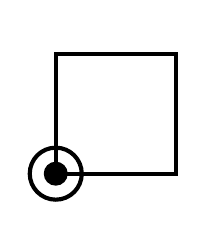
\begin{tikzpicture}[x=1in, y=1in]
\draw[line width=1.4pt] (0,0.13) rectangle (0.6,0.73);
\fill (0,0.13) circle (0.06);
\draw[line width=1.5pt] (0,0.13) circle (0.13);
\path (0,-0) rectangle (0.6,0.86);
\end{tikzpicture}
\end{center}
\begin{center}
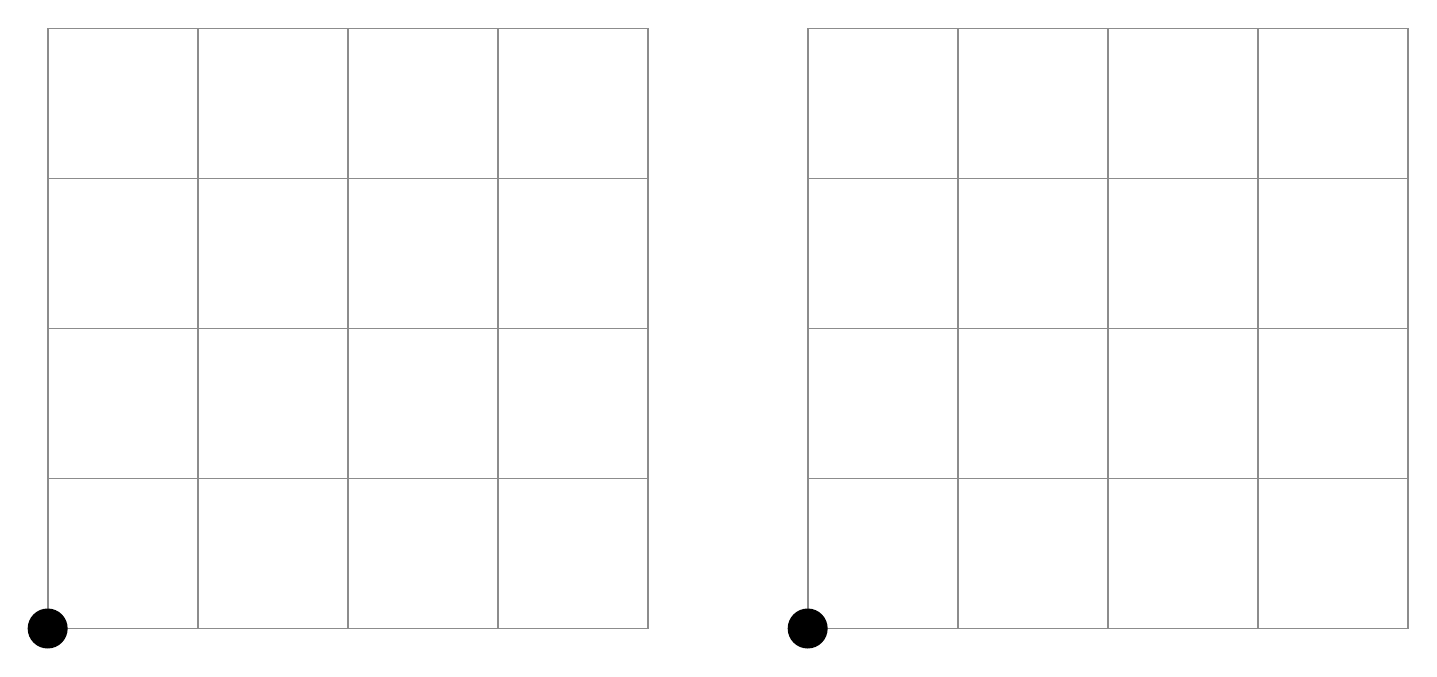
\begin{tikzpicture}[x=1in, y=1in]
\draw[black!45, line width=0.6pt] (0,0) -- (0,3);
\draw[black!45, line width=0.6pt] (0.75,0) -- (0.75,3);
\draw[black!45, line width=0.6pt] (1.5,0) -- (1.5,3);
\draw[black!45, line width=0.6pt] (2.25,0) -- (2.25,3);
\draw[black!45, line width=0.6pt] (3,0) -- (3,3);
\draw[black!45, line width=0.6pt] (0,0) -- (3,0);
\draw[black!45, line width=0.6pt] (0,0.75) -- (3,0.75);
\draw[black!45, line width=0.6pt] (0,1.5) -- (3,1.5);
\draw[black!45, line width=0.6pt] (0,2.25) -- (3,2.25);
\draw[black!45, line width=0.6pt] (0,3) -- (3,3);
\fill (0,0) circle (0.1);
\draw[black!45, line width=0.6pt] (3.8,0) -- (3.8,3);
\draw[black!45, line width=0.6pt] (4.55,0) -- (4.55,3);
\draw[black!45, line width=0.6pt] (5.3,0) -- (5.3,3);
\draw[black!45, line width=0.6pt] (6.05,0) -- (6.05,3);
\draw[black!45, line width=0.6pt] (6.8,0) -- (6.8,3);
\draw[black!45, line width=0.6pt] (3.8,0) -- (6.8,0);
\draw[black!45, line width=0.6pt] (3.8,0.75) -- (6.8,0.75);
\draw[black!45, line width=0.6pt] (3.8,1.5) -- (6.8,1.5);
\draw[black!45, line width=0.6pt] (3.8,2.25) -- (6.8,2.25);
\draw[black!45, line width=0.6pt] (3.8,3) -- (6.8,3);
\fill (3.8,0) circle (0.1);
\path (0,-0) rectangle (6.8,3);
\end{tikzpicture}
\end{center}
\vspace*{0.15in}
\begin{center}
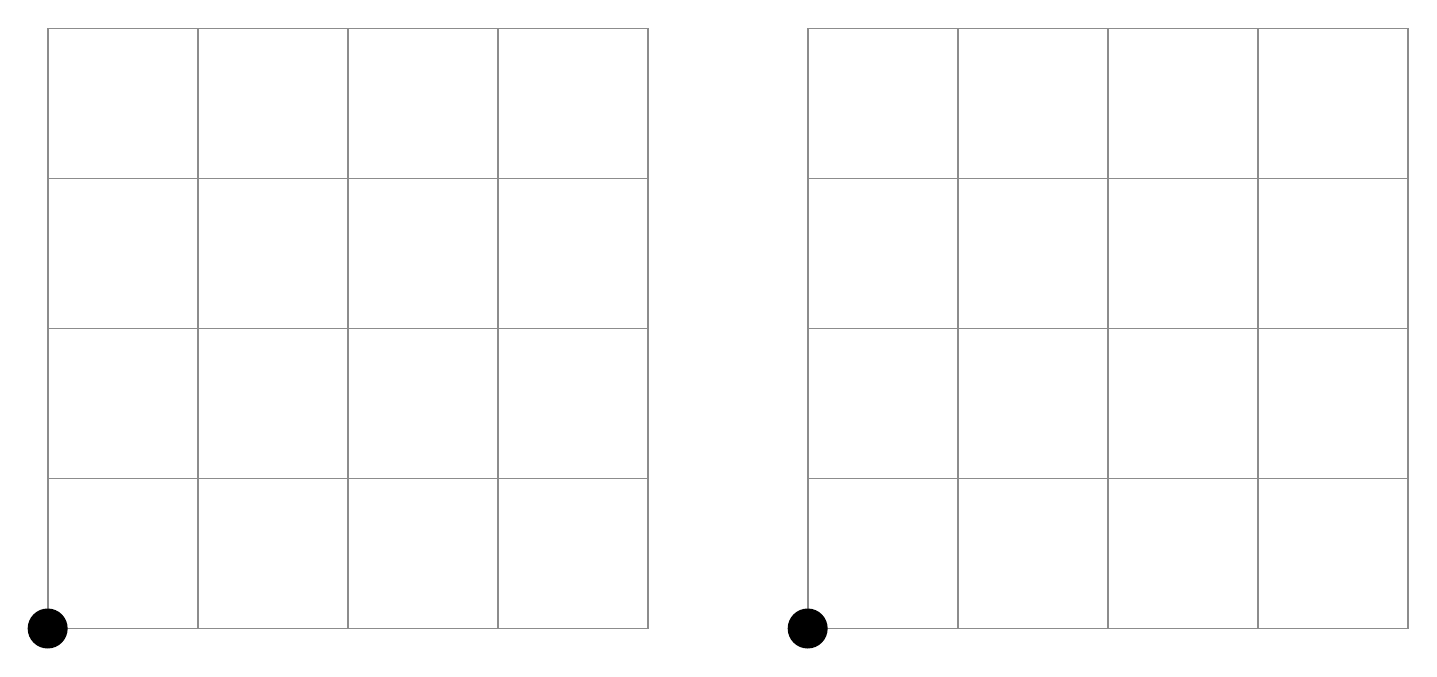
\begin{tikzpicture}[x=1in, y=1in]
\draw[black!45, line width=0.6pt] (0,0) -- (0,3);
\draw[black!45, line width=0.6pt] (0.75,0) -- (0.75,3);
\draw[black!45, line width=0.6pt] (1.5,0) -- (1.5,3);
\draw[black!45, line width=0.6pt] (2.25,0) -- (2.25,3);
\draw[black!45, line width=0.6pt] (3,0) -- (3,3);
\draw[black!45, line width=0.6pt] (0,0) -- (3,0);
\draw[black!45, line width=0.6pt] (0,0.75) -- (3,0.75);
\draw[black!45, line width=0.6pt] (0,1.5) -- (3,1.5);
\draw[black!45, line width=0.6pt] (0,2.25) -- (3,2.25);
\draw[black!45, line width=0.6pt] (0,3) -- (3,3);
\fill (0,0) circle (0.1);
\draw[black!45, line width=0.6pt] (3.8,0) -- (3.8,3);
\draw[black!45, line width=0.6pt] (4.55,0) -- (4.55,3);
\draw[black!45, line width=0.6pt] (5.3,0) -- (5.3,3);
\draw[black!45, line width=0.6pt] (6.05,0) -- (6.05,3);
\draw[black!45, line width=0.6pt] (6.8,0) -- (6.8,3);
\draw[black!45, line width=0.6pt] (3.8,0) -- (6.8,0);
\draw[black!45, line width=0.6pt] (3.8,0.75) -- (6.8,0.75);
\draw[black!45, line width=0.6pt] (3.8,1.5) -- (6.8,1.5);
\draw[black!45, line width=0.6pt] (3.8,2.25) -- (6.8,2.25);
\draw[black!45, line width=0.6pt] (3.8,3) -- (6.8,3);
\fill (3.8,0) circle (0.1);
\path (0,-0) rectangle (6.8,3);
\end{tikzpicture}
\end{center}
\newpage
\prob{7} With a ruler, draw a straight line from the dot to the far corner of each big square. Cut out the square and fold it on the dashed lines, with the dot on top. Hold it up to the light, and draw the line you see on the small table next to it.
\vspace*{0.2in}
\begin{center}
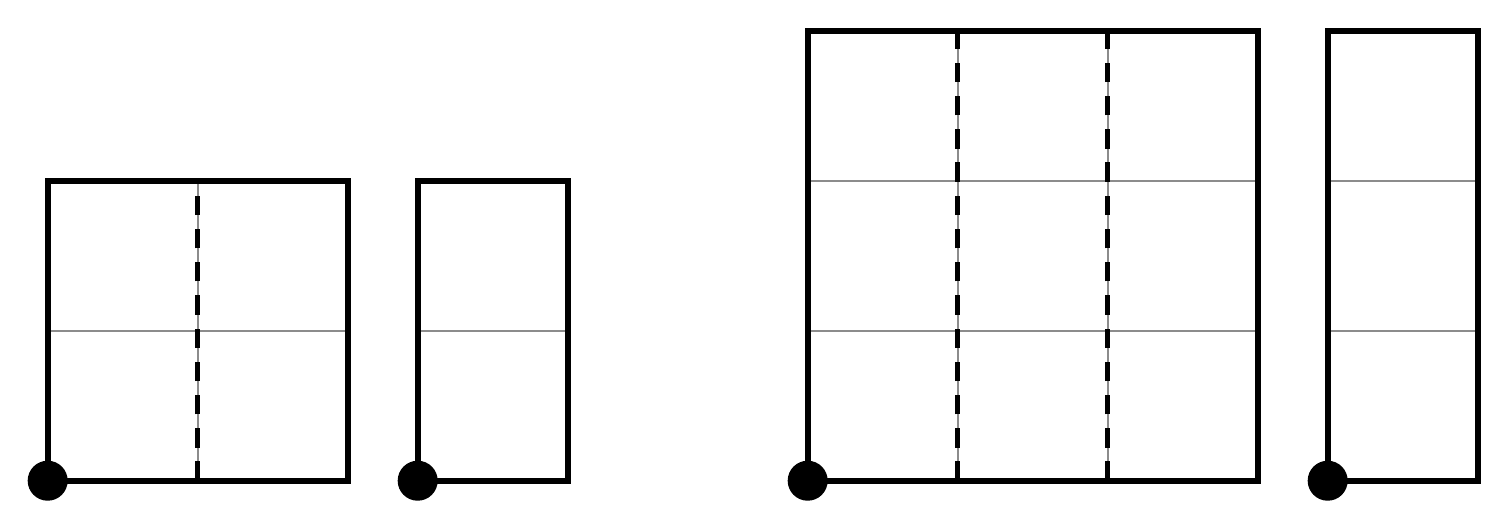
\begin{tikzpicture}[x=1in, y=1in]
\draw[black!45, line width=0.6pt] (0,0) -- (0,1.5);
\draw[black!45, line width=0.6pt] (0.75,0) -- (0.75,1.5);
\draw[black!45, line width=0.6pt] (1.5,0) -- (1.5,1.5);
\draw[black!45, line width=0.6pt] (0,0) -- (1.5,0);
\draw[black!45, line width=0.6pt] (0,0.75) -- (1.5,0.75);
\draw[black!45, line width=0.6pt] (0,1.5) -- (1.5,1.5);
\draw[line width=1.6pt, dash pattern=on 7pt off 5pt] (0.75,0) -- (0.75,1.5);
\draw[line width=2.2pt] (0,0) rectangle (1.5,1.5);
\fill (0,0) circle (0.1);
\draw[black!45, line width=0.6pt] (1.85,0) -- (1.85,1.5);
\draw[black!45, line width=0.6pt] (2.6,0) -- (2.6,1.5);
\draw[black!45, line width=0.6pt] (1.85,0) -- (2.6,0);
\draw[black!45, line width=0.6pt] (1.85,0.75) -- (2.6,0.75);
\draw[black!45, line width=0.6pt] (1.85,1.5) -- (2.6,1.5);
\draw[line width=2.2pt] (1.85,0) rectangle (2.6,1.5);
\fill (1.85,0) circle (0.1);
\draw[black!45, line width=0.6pt] (3.8,0) -- (3.8,2.25);
\draw[black!45, line width=0.6pt] (4.55,0) -- (4.55,2.25);
\draw[black!45, line width=0.6pt] (5.3,0) -- (5.3,2.25);
\draw[black!45, line width=0.6pt] (6.05,0) -- (6.05,2.25);
\draw[black!45, line width=0.6pt] (3.8,0) -- (6.05,0);
\draw[black!45, line width=0.6pt] (3.8,0.75) -- (6.05,0.75);
\draw[black!45, line width=0.6pt] (3.8,1.5) -- (6.05,1.5);
\draw[black!45, line width=0.6pt] (3.8,2.25) -- (6.05,2.25);
\draw[line width=1.6pt, dash pattern=on 7pt off 5pt] (4.55,0) -- (4.55,2.25);
\draw[line width=1.6pt, dash pattern=on 7pt off 5pt] (5.3,0) -- (5.3,2.25);
\draw[line width=2.2pt] (3.8,0) rectangle (6.05,2.25);
\fill (3.8,0) circle (0.1);
\draw[black!45, line width=0.6pt] (6.4,0) -- (6.4,2.25);
\draw[black!45, line width=0.6pt] (7.15,0) -- (7.15,2.25);
\draw[black!45, line width=0.6pt] (6.4,0) -- (7.15,0);
\draw[black!45, line width=0.6pt] (6.4,0.75) -- (7.15,0.75);
\draw[black!45, line width=0.6pt] (6.4,1.5) -- (7.15,1.5);
\draw[black!45, line width=0.6pt] (6.4,2.25) -- (7.15,2.25);
\draw[line width=2.2pt] (6.4,0) rectangle (7.15,2.25);
\fill (6.4,0) circle (0.1);
\path (0,-0) rectangle (7.15,2.25);
\end{tikzpicture}
\end{center}
\vspace*{0.45in}
\begin{center}
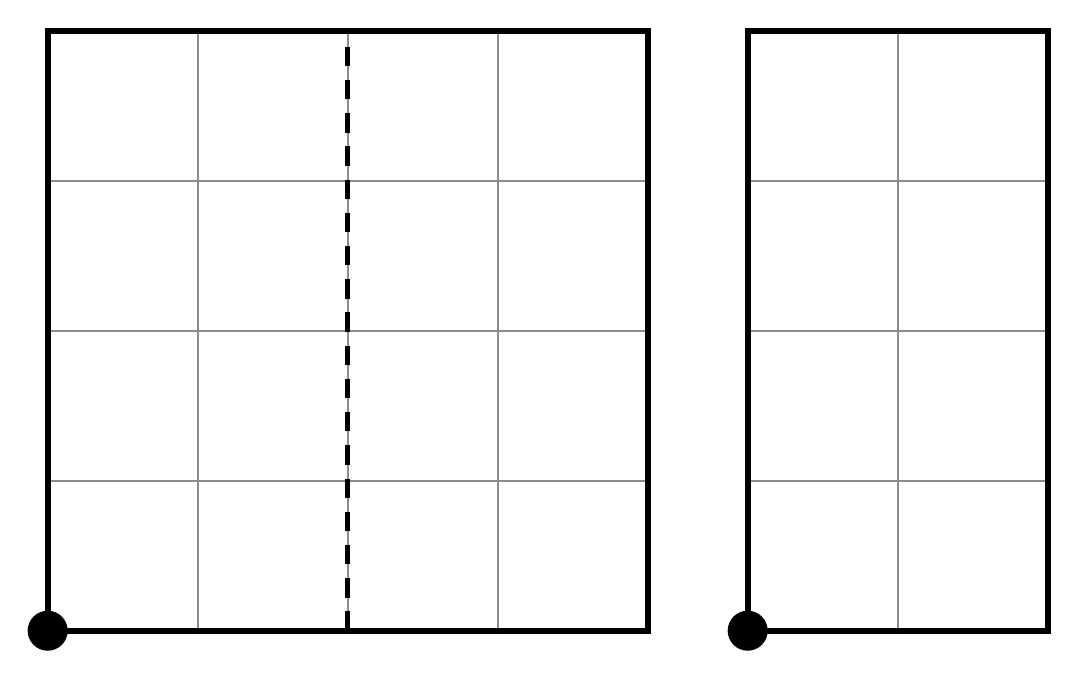
\begin{tikzpicture}[x=1in, y=1in]
\draw[black!45, line width=0.6pt] (0,0) -- (0,3);
\draw[black!45, line width=0.6pt] (0.75,0) -- (0.75,3);
\draw[black!45, line width=0.6pt] (1.5,0) -- (1.5,3);
\draw[black!45, line width=0.6pt] (2.25,0) -- (2.25,3);
\draw[black!45, line width=0.6pt] (3,0) -- (3,3);
\draw[black!45, line width=0.6pt] (0,0) -- (3,0);
\draw[black!45, line width=0.6pt] (0,0.75) -- (3,0.75);
\draw[black!45, line width=0.6pt] (0,1.5) -- (3,1.5);
\draw[black!45, line width=0.6pt] (0,2.25) -- (3,2.25);
\draw[black!45, line width=0.6pt] (0,3) -- (3,3);
\draw[line width=1.6pt, dash pattern=on 7pt off 5pt] (1.5,0) -- (1.5,3);
\draw[line width=2.2pt] (0,0) rectangle (3,3);
\fill (0,0) circle (0.1);
\draw[black!45, line width=0.6pt] (3.5,0) -- (3.5,3);
\draw[black!45, line width=0.6pt] (4.25,0) -- (4.25,3);
\draw[black!45, line width=0.6pt] (5,0) -- (5,3);
\draw[black!45, line width=0.6pt] (3.5,0) -- (5,0);
\draw[black!45, line width=0.6pt] (3.5,0.75) -- (5,0.75);
\draw[black!45, line width=0.6pt] (3.5,1.5) -- (5,1.5);
\draw[black!45, line width=0.6pt] (3.5,2.25) -- (5,2.25);
\draw[black!45, line width=0.6pt] (3.5,3) -- (5,3);
\draw[line width=2.2pt] (3.5,0) rectangle (5,3);
\fill (3.5,0) circle (0.1);
\path (0,-0) rectangle (5,3);
\end{tikzpicture}
\end{center}
\end{document}
